\section{Механизмы шифрования данных в Android}

\subsection*{Полнодисковое шифрование (FDE)}

Впервые полнодисковое шифрование (full disk encryption — FDE) пытались внедрить
еще в планшетной версии Android 3.0 Honeycomb. Тогда вместе с ядром Linux
2.6.36 в ней появился модуль dm-crypt, обеспечивающий возможность шифрования на
любом блочном устройстве хранения данных (включая NAND Flash). В универсальной
четвертой версии Android шифрование также было доступно, однако для большинства
оно оставалось невостребованной опцией. Из-за отсутствия программных
оптимизаций и низкой скорости встраиваемых процессоров того времени включение
шифрования приводило к падению производительности ввода-вывода в 6–8 раз на
топовых моделях и до 20 раз на бюджетных.

Исправить ситуацию удалось только с появлением 64-битных процессоров, имеющих
отдельный набор инструкций для ускорения криптографических вычислений. Поэтому
обязательным шифрование в Android стало только с версии 5.0,
предустанавливаемой на устройства с современными однокристальными системами.

Именно в пятой версии Андроида появился флаг forceencrypt fstab, указывающий на
необходимость активации шифрования при первом включении устройства. Обрати
внимание: есть принципиальная разница между тем, было ли устройство обновлено
до Android 5.x или новее либо сразу выпускалось с такой версией. Во втором
случае шифрование данных будет выполняться всегда. В первом варианте (при
обновлении) оно останется опциональным и может быть отключено сбросом до
заводских настроек (factory reset).

В общем случае для полнодискового шифрования в Android используются три битовые
последовательности: мастер-ключ, соль и пользовательский пин-код. Мастер-ключ и
соль генерируются автоматически, а пин-код вводится владельцем устройства. Роль
пин-кода может также выполнять пароль, графический ключ или любой другой
«секрет» — для процессора это все равно битовая последовательность, причем
довольно короткая.

Пользовательские данные шифруются мастер-ключом, а соль и пин-код служат только
для того, чтобы хранить сам мастер-ключ в зашифрованном виде. Поэтому смена
пароля не приводит к перешифровке всех данных. Ключ всегда остается один и тот
же (сгенерированный изначально), а новый пароль лишь меняет его
криптографическую оболочку. Разберем эту схему подробнее.

При первом включении устройство с предустановленной ОС Android 5.0 и выше
генерирует псевдослучайный 128-разрядный ключ. Его называют мастер-ключом, или
DEK (device encryption key). Помимо DEK, также генерируется еще одно
псевдослучайное 128-битное число (соль), а пользователя просят ввести пароль.

Именно с помощью DEK в конечном счете шифруются все данные на пользовательском
разделе /data. Как именно выглядит этот ключ, владелец устройства не знает. Он
никогда не вводит его и даже не может считать штатными средствами.

В ранних версиях Android (до 5.0) мастер-ключ и настройки шифрования хранились
в отдельной незашифрованной структуре crypto footer (упрощенный аналог LUKS) в
начале зашифрованного раздела data. Сам DEX шифровался другим ключом,
вычисляемым на основе пользовательского пароля и соли.

Такой способ не обеспечивал защиту от брутфорса мастер-ключа на внешних
вычислительных системах, поэтому в Android 5.0 и выше появилось новое
требование к производителям устройств: предоставлять на аппаратном уровне
защищенное хранилище ключей. Дополнительно DEK стал подписываться с
использованием еще одного ключа (HBK — hardware-bound private key),
специфичного для данного устройства. Он захардкожен на этапе производства и не
доступен ни одному пользовательскому процессу.

Как хранение ключа, так и все ключевые криптографические процедуры в
современных версиях Android должны выполняться в изолированной среде,
недоступной пользователю и приложениям. На практике же это условие соблюдается
не всегда, поскольку Android работает на совершенно разных платформах.
Концептуально их три: ARM, Intel x86 и MIPS. В каждой из них есть свои
архитектурные ветвления, которые добавляют путаницы. Более того, на базе одних
и тех же ядер (например, ARM Cortex-A53) каждый производитель, обладающий
лицензией на архитектуру (architectural license), может сделать свою версию
однокристальной системы с любыми нестандартными свойствами.

Именно из-за такого разнообразия платформ Google до сих пор не может обеспечить
единый фундамент для шифрования, как это сделала Apple еще в 2013 году (см.
Secure Enclave). Сегодня в устройствах под управлением Android либо защищенного
хранилища ключей нет вовсе, либо оно не имеет надежной реализации.

\subsubsection*{Как работает FDE}

Поэтапно схема создания ключей для шифрования пользовательских данных в Android 5.0 и выше выглядит так:

\begin{enumerate}
    \item Гаджет при первом включении генерирует два числа длиной 128 бит. В
    дальнейшем они используются как мастер-ключ и соль.
    \item Пользователя просят задать пароль.
    \item На основе введенного пароля функция scrypt запускает формирование
    первого промежуточного ключа (IK1) длиной 256 бит.
    \item IK1 дополняется нулями так, чтобы соответствовать по длине
    аппаратному ключу HBK.
    \item Модифицированный ключ IK1 подписывается ключом HBK.
    \item Подписанный ключ IK1 используется как второй промежуточный ключ (IK2).
    \item Функция scrypt запускает формирование третьего промежуточного ключа
    (IK3), используя для его генерации IK2 и соль как входные аргументы.
    \item Первые 128 бит IK3 используются как KEK (key encryption key — ключ
    шифрования мастер-ключа).
    \item Мастер-ключ шифруется ключом KEK по алгоритму AES в режиме сцепления
    блоков шифртекста (CBC). Поскольку в данном режиме одинаковые исходные
    блоки дают одинаковый шифртекст, для затруднения атаки на основе
    подобранного шифртекста в качестве данных первого блока используется
    случайная последовательность (вектор инициализации).
    \item Зашифрованный мастер-ключ сохраняется в аппаратно изолированной области.
\end{enumerate}

Мастер-ключ используется для шифрования всего содержимого пользовательского
раздела во встроенной памяти устройства. Для каждого сектора генерируется свой
вектор инициализации с солью и указанием номера сектора (ESSIV). При вводе
пользовательского пароля мастер-ключ расшифровывается, и далее пользовательские
данные автоматически расшифровываются в фоне.

Недоступность всех ключей для прямого считывания (например, запущенным на
устройстве скриптом) обеспечивается их обработкой только внутри изолированной
доверенной среды исполнения (trusted execution environment — TEE). В
процессорах архитектуры ARM роль TEE выполняет TrustZone, которая обеспечивает
контроль целостности данных, их защищенное хранение и изолированное выполнение
кода. В ней же хранятся и промежуточные значения, вычисляемые функцией
формирования ключа.

\begin{figure}
    \centering
    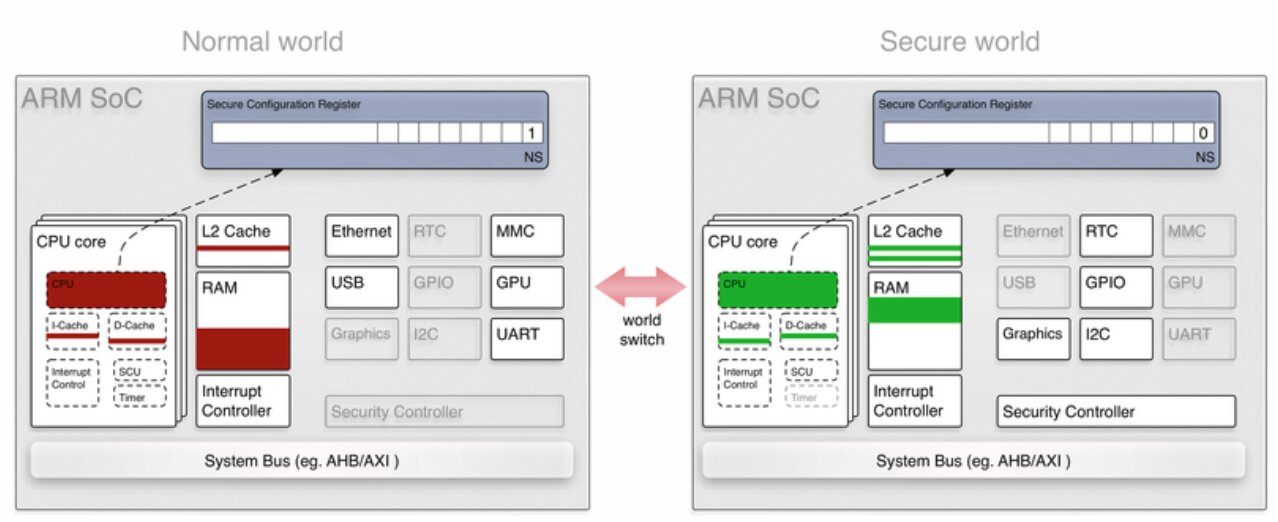
\includegraphics[scale=0.3]{inc/trustzone.jpg}
    \caption{ Схема организации доверенной среды}
    \label{fig:fig02}
\end{figure}

\subsection*{Пофайловое шифрование (FBE)}

В Android 7.0 появилась принципиально новая функция — пофайловое шифрование
(file based encryption — FBE), которое выполняется с использованием
возможностей файловой системы ext4. Новая реализация шифрования требует наличия
аппаратно изолированной среды (trusted execution environment) с поддержкой API
Keymaster 1.0 (старые версии 0.xx не годятся). Выполнение алгоритма AES
процессором должно обеспечивать расшифровку данных со скоростью не менее 50
Мбайт/с.

При использовании FBE каждый файл может быть зашифрован своим ключом и
расшифрован независимо от остальных. Эта функция работает вместе с другой
новинкой седьмого «Андроида» — прямой загрузкой (Direct Boot).

Direct Boot API обеспечивает более деликатное отделение приватных данных от
прочих файлов. Он предоставляет ту функциональность, которая была недоступна
при использовании полнодискового шифрования.

До появления Android 7.0 при активации FDE все данные хранились зашифрованными
общим паролем, поэтому смартфоном невозможно было пользоваться до ввода пароля.
Теперь же отдельные приложения (например, будильник) можно сделать доступными
прямо на экране блокировки. Они будут работать без авторизации со своими
заранее заданными ограничениями, а все пользовательские данные тем временем
останутся зашифрованными.

На устройстве с активным пофайловым шифрованием у пользователя появляется две
области хранения данных приложений: зашифрованная отдельным паролем (Credential
Encrypted — CE) и зашифрованная общим ключом устройства (Device Encrypted —
DE). При отключении FBE обе области (CE и DE) остаются открытыми для любого
приложения. При активном шифровании файлы области CE расшифровываются только
после ввода пользовательского пароля. Файлы DE могут быть расшифрованы сразу
после загрузки. Заодно раздельные пароли на каждый аккаунт позволяют создавать
на одном устройстве несколько изолированных пользовательских учеток — например,
для детей и ведущих себя подобно детям сотрудников.

Шифрование области CE происходит по алгоритму AES, но уже в другом режиме —
XTS. Он разрабатывался специально для шифрования на блочных устройствах и не
имеет типичных для режима CBC уязвимостей. В частности, XTS не позволяет
определить точку изменения данных, не подвержен утечке данных, устойчив к
атакам подмены и перемещения.

С другой стороны, FBE уязвим к side channel атакам, так как, несмотря на
шифрование файлов и их имен, он оставляет открытыми метаданные, что можно
использовать для выяснения типа хранимой информации и идентификации
пользователя устройства.

\subsection*{Android Keystore}

Одним из ключевых элементов обеспечения криптографической безопасности на
платформе Android является система \textbf{Android Keystore}. Она предназначена
для безопасного создания, хранения и использования криптографических ключей без
необходимости их извлечения в открытом виде из защищённого хранилища. Это
позволяет приложениям использовать шифрование, цифровую подпись и проверку
целостности данных без прямого доступа к самим ключам.

\subsubsection*{Назначение и архитектура}

Основная цель Android Keystore --- защитить криптографические ключи от
несанкционированного доступа и обеспечить их изоляцию от остальной части
операционной системы и приложений. Система Keystore реализована как сервис,
работающий внутри Android Framework и взаимодействующий с низкоуровневыми
компонентами устройства. На большинстве современных устройств Keystore
использует аппаратную защиту, включая:

\begin{itemize}
    \item \textbf{Trusted Execution Environment (TEE)} --- изолированная среда
    внутри процессора, в которой выполняются критические операции, включая
    криптографические.
    \item \textbf{Hardware Security Module (HSM)} --- специализированный
    аппаратный модуль для управления ключами (например, чип Titan M в
    устройствах Google Pixel).
    \item \textbf{Secure Element (SE)} --- отдельный чип, физически
    изолированный от основной системы, применяемый в некоторых устройствах для
    хранения ключей и выполнения безопасных операций.
\end{itemize}

\subsubsection*{Принцип работы}

Работа с Keystore происходит с помощью API, предоставляемого Android SDK.
Приложения могут:

\begin{itemize}
    \item Генерировать ключи асимметричного и симметричного шифрования.
    \item Выполнять операции шифрования и расшифровки данных.
    \item Подписывать и проверять цифровые подписи.
    \item Задавать условия использования ключей (например, только при разблокированном экране или только после аутентификации пользователя).
\end{itemize}

Важно, что в большинстве случаев приложение не может извлечь ключ из Keystore
--- оно может лишь передавать данные на шифрование, а сам ключ остаётся
изолированным.

\subsubsection*{Типы поддерживаемых ключей}

Android Keystore поддерживает следующие алгоритмы:

\begin{itemize}
    \item \textbf{RSA} --- асимметричное шифрование, цифровые подписи.
    \item \textbf{EC (Elliptic Curve)} --- более эффективная альтернатива RSA для цифровой подписи.
    \item \textbf{AES} --- симметричное шифрование (начиная с Android 6.0).
    \item \textbf{HMAC} --- генерация и проверка MAC-кодов.
\end{itemize}

\subsection{Условия доступа и ограничения}

Разработчики могут задать параметры для каждого ключа при его создании:

\begin{itemize}
    \item Ключ может использоваться только после прохождения биометрической или PIN-аутентификации.
    \item Ограничение по времени жизни ключа.
    \item Возможность использования только в зашифрованной области (Credential Encrypted Storage).
    \item Возможность блокировки ключа после перезагрузки устройства.
\end{itemize}

Эти условия реализуются на уровне TEE или аппаратного модуля, что делает обход этих ограничений крайне сложным даже при наличии root-доступа.

\subsubsection*{Практическое применение}

Android Keystore активно используется как в системных приложениях, так и в
стороннем программном обеспечении. Типичные сценарии использования:

\begin{itemize}
    \item Защита учётных данных (токенов, паролей) с помощью шифрования.
    \item Хранение ключей для HTTPS-соединений и VPN.
    \item Цифровая подпись и верификация целостности данных.
    \item Реализация безопасной аутентификации пользователей.
\end{itemize}

Для разработчиков Google предоставляет библиотеку
\texttt{EncryptedSharedPreferences} и \texttt{EncryptedFile}, которые
используют Keystore для защиты данных на уровне приложений.

\subsubsection*{Недостатки и ограничения}

Несмотря на высокую степень защиты, Android Keystore имеет и определённые ограничения:

\begin{itemize}
    \item Не все устройства поддерживают аппаратную реализацию Keystore; в некоторых случаях ключи хранятся в программной области.
    \item Ограниченное количество операций в секунду при аппаратной реализации.
    \item При сбросе устройства все ключи удаляются (если не использован резервный механизм).
    \item Интерфейс API может отличаться в зависимости от версии Android и производителя.
\end{itemize}
